\chapter{Simultaneous Localization and Mapping}

Um das Ziel des exakten Matchings von Realität und generierter virtueller Realität zu erreichen, ist \glqq Camera Localization\grqq{}  die Schlüsseltechnologie für alle Augmented Reality Anwendungen (vgl. \cite{slam_mobile} S.1). Weiterhin ist es wichtig, die Umgebung zu kartographieren, um Projektionsflächen für virtuelle dreidimensionale Objekte zu finden. Eine mögliche Lösung für dieses Problem ist die Verwendung von SLAM. In den letzten 20 Jahren hat sich bei SLAM ein Trend gezeigt, bei dem Kameras als einzige exterozeptive Sensoren verwendet werden. Der Hauptgrund dafür ist die Fähigkeit eines Kamera-basierten Systems, Tiefeninformationen, Farben, Texturen und Helligkeiten zu erkennen, was beispielsweise Objekt- oder Gesichtserkennung ermöglicht. Darüber hinaus sind Kameras preiswert, leicht und haben einen geringen Stromverbrauch (vgl. \cite{survey} S.57). 

Erst in den letzten Jahren hat sich SLAM in Alltagsanwendungen profilieren können, hauptsächlich durch das Aufkommen von leistungsstarken Smartphones. Smartphones sind mobil und haben die nötige Rechenleistung um SLAM Algorithmen in Echtzeit auszuführen. Dies hat zu einer Erweiterung der Forschungsmöglichkeiten von SLAM basierten Ansätzen geführt und das Verfahren zu einer robusteren Technologie gemacht. Weiterhin verfügen Smartphones über eine Vielzahl an Sensoren, wie Beschleunigungssensor, Gyroskop, Magentometer oder GPS, mit denen die visuellen Daten ergänzt werden können, um die Map genauer und weniger anfällig für innere Drifteffekte zu machen, was jedoch wieder eigene komplexe Probleme bei der Verbindung von verschiedenen Sensordaten mit sich bringt (vgl. \cite{ar_slam} S.4). Folgende Tabelle gibt eine Übersicht an Software Development Kits, die SLAM implementiert haben, sowie die freie Verfügbarkeit deren Quelltext:

\begin{table}[h!]
\hskip-1.9cm
\begin{tabular}{|l|l|l|l|l|l|l|l|l|l|}
\hline
            & Vuforia & Wikitude & Metaio & ARToolKit & Kudan & EasyAR & MaxST & ARCore & ARKit \\ \hline
SLAM        &  \checkmark       &   \checkmark       &   \checkmark     &    x       &  \checkmark     &   \checkmark     &      \checkmark &   \checkmark     &    \checkmark   \\ \hline
Open Source &    x     &    x      &   x     &     \checkmark      &   x    &    x    &   x    &   \checkmark     &  x     \\ \hline
\end{tabular}
\end{table}

Die Verwendung von SLAM im mobilen Bereich hat jedoch einige Probleme zu meistern. Durch die Ungenauigkeiten der absoluten Lokalisierung ist es schwierig, kontextsensitive Augmentation zu erzeugen. Auch wenn es möglich ist, bekannte Objekte im Raum während des Trackings zu bestimmen und die Information um diese herum zu zeigen, ist es fast unmöglich, den kompletten Raum einer Szenerie zu bestimmen. Das zweite Problem liegt in der Ergonomie und Benutzbarkeit der Anwendung durch den Endbenutzer. Typischerweise soll ein Endverbraucher keinem komplexen Protokoll folgen müssen, um sich selbst in der Szene zu lokalisieren. Das System benötigt also ein Verfahren zur schnellen und robusten Lokalisierung im Raum (vgl. \cite{slam_mobile} S.1).

SLAM als Problemstellung ist die Auswertung einer unbekannten Umgebung und Erstellung einer Karte, während gleichzeitig die lokale Position innerhalb dieser Karte bestimmt wird. Die Lösung dieses SLAM Problems war vor allem in der Robotik eine fundamentale Aufgabe der letzten zwei Jahrzehnte. Dabei ist SLAM ein Alltagsproblem: das Problem der räumlichen Erkundung. Jeder Mensch und jedes Tier hat dies gemeistert und benutzt es unterbewusst zur Navigation in unserer räumlichen Umgebung. Wichtige Anwendungsbereiche von SLAM sind die automatische Fahrzeugsteuerung auf unbekanntem Terrain, Rettungseinsätze in Umgebungen mit hohem Risiko, planetarische, terrestrische oder ozeanische Exploration, Augmented Reality Anwendungen, visuelle Überwachungssysteme oder Anwendungen in der Medizin. Die Lösung dieses Problems ist sehr komplex, wenn es für einen Roboter oder für Smartphones automatisiert ausgeführt werden soll. Durch das beherrschen dieser Technik können beispielsweise Roboter oder Fahrzeuge wirklich autonom gesteuert werden. Bei SLAM wird die Bewegung des Objekts an sich durch den Raum und die Position aller zur Positionsbestimmung notwendigen Merkmale berechnet, ohne vorheriges Wissen über Position oder Lage im Raum (vgl. \cite{slam} S. 1-2, \cite{survey} S.56).

Dabei benötigt man mindestens einen exterozeptiven Sensor um Informationen der Umgebung zu sammeln.
SLAM besteht aus drei grundlegenden Operationen, die iterativ pro Zeitintervall ausgeführt werden (vgl. \cite{ekf_slam} S.3):

\textbf{Die Kamera bewegt sich} und erreicht eine neue Position in der Umwelt. Diese Bewegung erzeugt durch unvermeidbares Rauschen und Fehler Ungewissheit über die wirkliche absolute Position. Eine automatisierte Lösung benötigt ein mathematisches Modell für diese Bewegung. Dies ist das \glqq\textit{Motion Model}\grqq{}.

\textbf{Neue Features werden in der Umgebung entdeckt}, welche in die Umgebungskarte aufgenommen werden müssen. Diese Features heißen \glqq Landmarks\grqq{}. Da die Position der Landmarks genauso wie die aktuelle Position der Kamera, durch Fehler in den exterozeptiven Sensoren ungewiss ist, müssen diese beiden Faktoren passend arrangiert werden. Eine automatisierte Lösung benötigt ein mathematisches Modell, das die Position der Landmarks anhand der Sensordaten bestimmt. Dies ist das \glqq{}\textit{Inverse Oberservation Model}\grqq{}.

\textbf{Schon gemappte Landmarks werden entdeckt}, welche dann verwendet werden, um die eigene Position, sowie die aller anderen Landmarks, zu korrigieren. Diese Operation reduziert die Unsicherheit über den aktuellen Standort, sowie die der Landmarks. Die automatisierte Lösung erfordert ein mathemathisches Modell, um die Werte der Messungen aus den prognostizierten Positionen der Landmarks und der aktuellen Position der Kamera zu berechnen. Dies ist das \glqq \textit{Direct Observation Model}\grqq

Mit den drei Modellen ist es möglich, eine automatisierte Lösung für SLAM zu entwerfen. Die Lösung muss diese drei Modelle verbinden und alle Daten korrekt, organisiert und aktuell halten, sowie die korrekten Entscheidungen bei jedem Iterationsschritt machen (vgl. \cite{ekf_slam} S.2-3).

\begin{figure}[H]
	\centering
	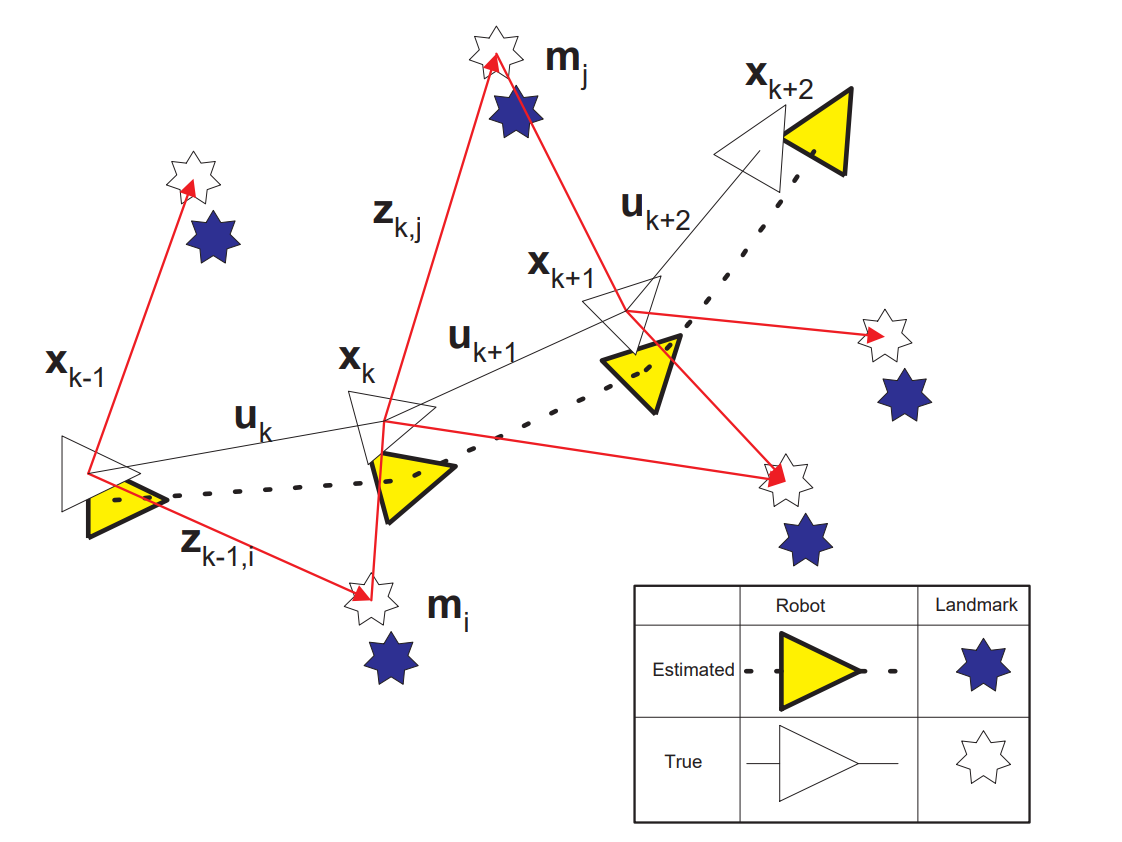
\includegraphics[scale=0.55]{slam_problem.png}
	\caption{Das SLAM Problem: Die wahren absoluten Positionen der extrahierten Features sind nie wirklich bekannt. Bildquelle \cite{slam}}
\end{figure} 

Eine erfolgreiche Lösung des SLAM Problems setzt weiterhin die Lösung des \glqq Loop Closure Detection\grqq{} Problems voraus. Dabei müssen bereits besuchte Orte und Landmarks in einer beliebig großen Karte erkannt werden. Eins der größten Hindernisse, wenn es um die Skalierbarkeit der Lösung des SLAM Problems geht, ist die mögliche Komplexität von großen Karten. Wichtig ist, dass die Loop Closure Detection keine Falsch-Positiven Ergebnisse liefert, da dies die Integrität und Korrektheit der kompletten Karte beeinflussen würde (vgl. \cite{ar_slam} S.4, siehe Kapitel 4.1).

Wie in Abbildung 4.1. erkennbar ist, bewegt sich in diesem Beispiel ein Roboter durch eine unbekannte Umgebung und nimmt mit seinem Sensor Features der näheren Objekte (Landmarks) auf. Wobei $x_k$ der Vektor des Roboters,  $u_k$ der Bewegungsvektor, $m_i$ der Vektor des Landmarks und $z_ik$ die Oberservation eines Landmarks durch den Roboter zur Zeit $k$ sind. Wie man sehen kann, ist der Fehler zwischen echten und geschätzten Landmarks bei allen geschätzten Landmarks ähnlich, was an der initialen Betrachtung der Umgebung liegt. Zu diesem Zeitpunk wird nur das erste Feature erkannt. Daraus kann man schließen, dass die Fehler in der Schätzung der Landmarkpositionen korrelieren. Praktisch bedeutet dies, dass die relative Position zweier Landmarks, $m_i - m_j$ zueinander sehr genau sein kann, auch wenn die absolute Position sehr ungenau ist (vgl. \cite{slam} S.2).

\begin{figure}[H]
	\centering
	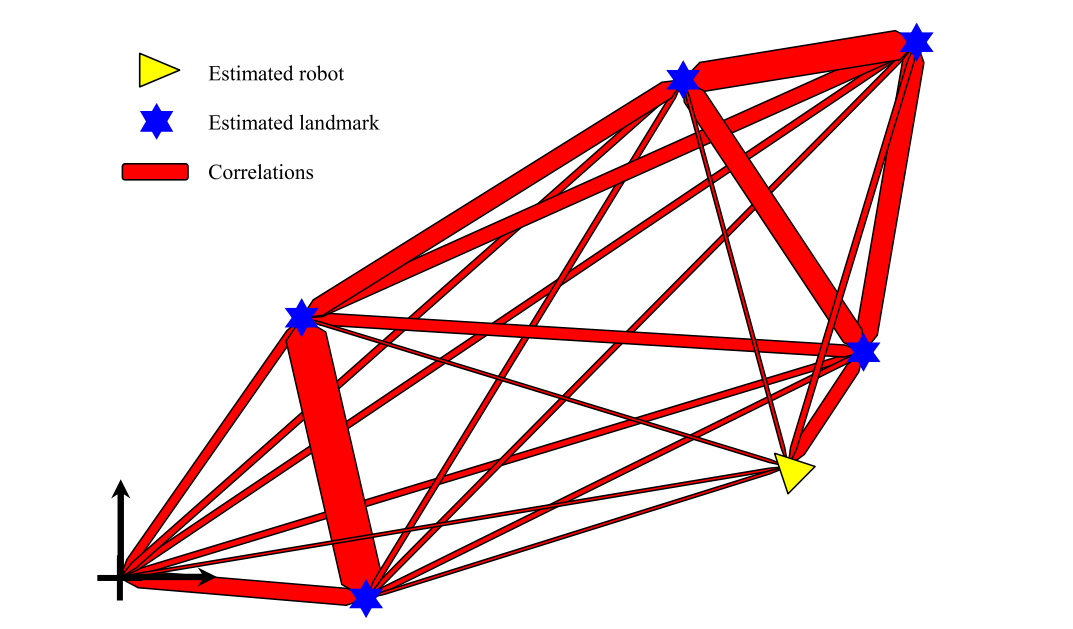
\includegraphics[scale=0.6]{slam_springs.png}
	\caption{Die Landmarks sind durch \glqq Federn\grqq{} verbunden, welche die Korrelation zwischen ihnen darstellen.  Bildquelle \cite{slam}}
\end{figure}  


Je mehr Landmarks in das Modell aufgenommen werden, desto besser wird das Modell der relativen Positionen, egal wie sich der Roboter bewegt. Dieser Prozess wird in Abbildung 4.2. veranschaulicht.

Während sich der Roboter durch die Umgebung bewegt, werden die Korrelationen stetig aktualisiert. Je mehr Beobachtungen über die Umwelt gemacht werden, desto steifer werden die Federn in diesem Modell. Im Nachhinein werden neue Beobachtungen von Landmarks durch das ganze Netzwerk propagiert und je nach Input, kleinere oder größere Anpassungen vorgenommen.

\section{Loop Closure Detection}

Die \glqq Loop Closure Detection\grqq{} (Schleifenerkennung) besteht in der Erkennung von bereits besuchten Orten nach der zyklischen Erkundung der Umwelt und nach beliebiger Länge des Weges. Dies ist eins der größten Hindernisse, um SLAM im großen Maßstab zu verwenden, da kritische Fehler vermieden werden müssen, die schon durch ein falsch-positives Ergebnis entstehen.

\begin{figure}[H]
	\centering
	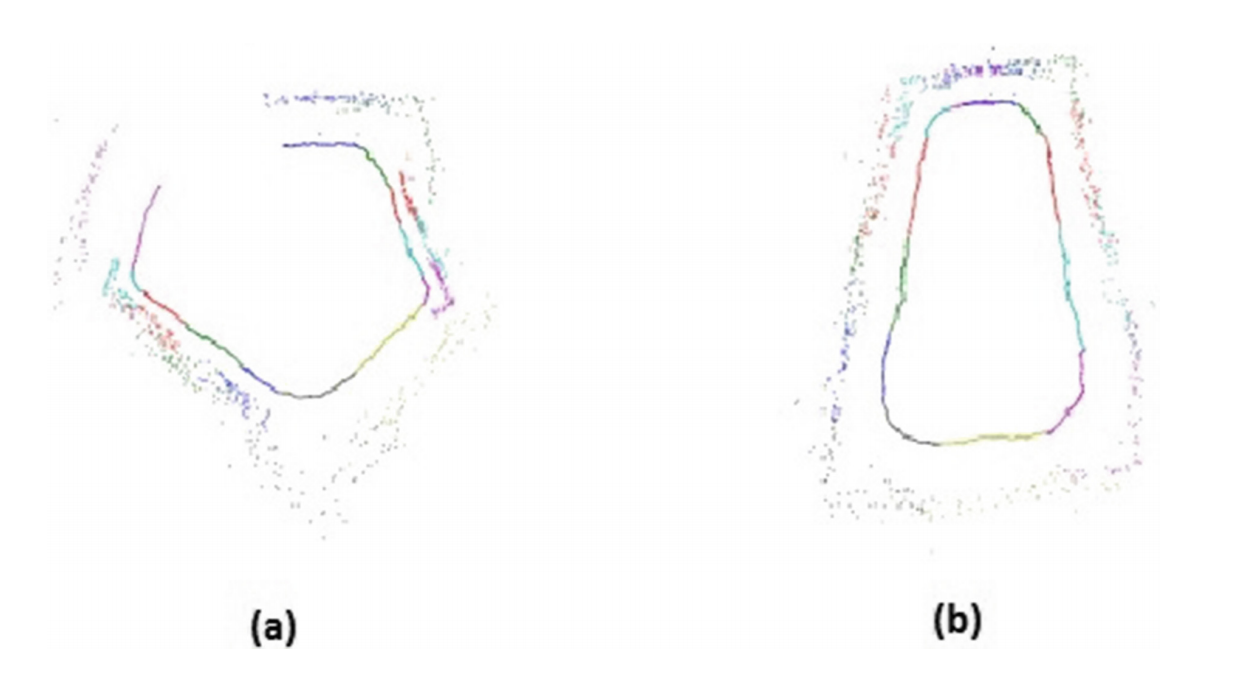
\includegraphics[scale=0.53]{loop.png}
	\caption{ Lösung des SLAM Problems ohne (a) und mit (b) einem Loop Closure Algorithmus. Die innere Kurve ist der Pfad des mobilen Systems, die äußeren Punkte stellen die Features in der Karte dar. Bildquelle \cite{loop_closure}}
\end{figure}  

Es ergibt sich ein weiteres Problem, das \glqq Perceptual Aliasing\grqq{} genannt wird und bei dem zwei verschiedene Orte aus der Umgebung als ein gleicher Ort erkannt werden. Dies stellt vor allem bei sich wiederholenden Features in der Umgebung, wie Fluren, ähnlichen architektonischen Elementen oder Zonen mit vielen Büschen oder Bäumen, ein großes Problem dar. Eine gute Methode zur Schleifenerkennung darf keine falsch-positiven Ergebnisse und nur ein Minimum an falsch-negativen Ergebnissen liefern. Deshalb müssen alle Loop Closure Systeme auf eine Präzision von 100 \% abzielen. Dies wird benötigt, da ein einzelnes falsch-positives Ergebnis zu irreparablen Fehlern in der Erstellung der Karte führt. Falsch-negative hingegen reduzieren nur den Anteil der Rückrufquote, haben aber keinen Einfluss auf die Präzision der Genauigkeit der Karte (vgl. \cite{survey} S.64-65).



Algorithmen für die Schleifenerkennung lassen sich in drei Gruppen unterteilen (vgl. \cite{loop_closure} S.212):

\begin{itemize}
\item \textbf{map-to-map}: Die Schleifenerkennung erfolgt durch die Aufteilung der globalen Karte in Teilkarten und dem Finden von Übereinstimmungen zwischen diesen Teilkarten.

\item \textbf{image-to-map}: Die Suche wird anhand von Übereinstimmungen zwischen Bild und Karte ermöglicht und die Position des Systems wird dann in Bezug zur Karte wiederhergestellt.

\item \textbf{image-to-image}: Die Schleifenerkennung wird anhand von Bildfeatures zwischen verschiedenen Bildern durchgeführt.

\end{itemize}
Nach der Erkennung einer Schleife wird das globale Kartenmodell angepasst, um die gewonnenen Erkenntnisse in die Karte zu übernehmen (vgl. \cite{loop_closure} S.213).

\section{Visual SLAM}

Wenn Kameras als einziger exterozeptiver Sensor verwendet werden, spricht man von \glqq Visual SLAM\grqq{} oder \glqq Vision-Based SLAM\grqq{}. Viele visuelle SLAM Ansätze haben jedoch Probleme wenn sie unter folgenden Bedingungen eingesetzt werden:

\begin{itemize}
\item In externen, dynamischen Umgebungen
\item In Umgebungen mit sehr wenigen oder sehr vielen markanten Merkmalen
\item In sehr großflächigen Umgebungen
\item Bei sehr unregelmäßigen Bewegungen der Kamera
\item Bei partieller oder großflächiger Verdeckung des Sensors
\end{itemize}

Ein Schlüsselelement von erfolgreichen SLAM Systemen ist die Fähigkeit, trotz dieser Schwierigkeiten korrekt zu arbeiten (vgl. \cite{survey} S.56).

Lösungen für das visuelle SLAM Problem benötigen eine angemessene Repräsentation für die Observierungen der Landmarks, welche eine konsistente und schnelle Berechnung ermöglichen. Die geläufigste Repräsentation besteht in der Form einer Zustandsraumdarstellung mit gaußschem Rauschen, was zur Verwendung des \glqq Extended Kalman Filter\grqq{} (EKF) führt (vgl. \cite{slam} S. 2-4). Weitere gängige Lösungen für das SLAM Problem sind \glqq Maximum Likelihood Techniques\grqq{}, \glqq Sparse Extended Information Filters\grqq{} (SEIFs), \glqq Rao Blackwellized Particle Filters\grqq{} (RBPFs), \glqq FAST-SLAM\grqq{} und \glqq ORB-SLAM\grqq{} (vgl. \cite{rao} S. 2). Im folgenden wird der Extended Kalman Filter vorgestellt, der in vielen SLAM Systemen zum Einsatz gekommen ist, sowie seine Weiterentwicklungen FAST-SLAM und ORB-SLAM.
  
 

\section{Extended Kalman Filter - SLAM}
Eine der ersten Methoden zur Lösung des SLAM Problems war die Verwendung von Extendet Kalman Filter SLAM, welches um 1990 entwickelt wurde (\cite{orb_slam} S.1). Der Kalman Filter ist eine Schätzfunktion für das \glqq Linear-Quadratic-Problem\grqq{}, welches das Problem der Schätzung des augenblicklichen Zustands eines linearen dynamischen Systems, gestört durch weißes Rauschen, darstellt. Der Kalman Filter wird auch dazu verwendet, um die mögliche Zukunft von dynamischen Systemen vorherzusagen, die von Menschen nicht kontrolliert werden können, wie zum Beispiel die Flugbahn von Himmelskörpern oder der Kurs von gehandelten Rohstoffen (vgl. \cite{ekf} S.1).

Der Kalman Filter besteht aus drei Schritten. Zuerst wird eine Messung vorhergesagt, welche dann mit der realen Messung verglichen wird. Die resultierende Differenz wird mit der Varianz der Messung gewichtet, um daraus eine neue Schätzung des Zustands zu erhalten (vgl. \cite{slam_studi} S.13). Der Kalman Filter lässt sich jedoch nur auf lineare Systeme anwenden. Der Extended Kalman Filter verwendet für die Vorhersage der Messungen und der Zustände hingegen nicht-lineare Funktionen (vgl. \cite{slam_studi} S.16-17). Beim Extended Kalman Filter - SLAM ist die Map ein großer Stapel an Vektor und Sensordaten, sowie Zuständen von Landmarks.

\begin{equation}
  x =  \begin{bmatrix}
		R\\
		M
     	\end{bmatrix}
     = \begin{bmatrix}
		R\\
		L_1\\
		...\\
		L_n
     	\end{bmatrix}
\end{equation}

\( R\) ist der Zustand des Sensors und \( M = (L_1, ..., L_n)\) ist ein Set an Zuständen der Landmarks.
Beim Extended Kalman Filter wird die Karte durch eine gaußsche Variable modelliert, die den Mittelwert und die Kovarianzmatrix des Zustandsvektors verwendet, die jeweils durch \(\overline{x}\) und \(P\) beschrieben werden. Das Ziel ist es, die Map \{\(\overline{x}, P\)\} zu allen Zeiten auf dem aktuellen Stand zu halten.


\begin{equation}
  \overline{x} =  
  		\begin{bmatrix}
		\overline{R}\\
		\overline{M}
     	\end{bmatrix}
     = 
     	\begin{bmatrix}
		\overline{R}\\
		\overline{L_1}\\
		...\\
		\overline{L_n}
     	\end{bmatrix}
     	\quad\quad
     P = 
     	\begin{bmatrix}
		P_{RR} & P_{RM}\\
		P_{MR} & P_{MM}
     	\end{bmatrix}
     = 
     	\begin{bmatrix}
		P_{RR} & P_{RL1} & ... & P_{RLn}\\
		P_{L1R} & P_{L1L1} & ... & P_{L1Ln}\\
		... & ... & ... & ... \\
		P_{LnR} & P_{LnL1} & ... & P_{LnLn}
     	\end{bmatrix}
\end{equation}

Diese stochastische Karte wird durch die Vorhersage- und Korrekturprozesse des EKF in Stand gehalten. Um eine echte Erkundung der Umgebung zu erreichen, wird der EKF Algorithmus mit einem zusätzlichen Schritt der Landmark Erkennung und Initialisierung gestartet, bei dem neue Landmarks zu der Karte hinzugefügt werden. Die Landmark Initialisierung erfolgt durch eine Umkehrung der Bewertungsfunktion und der Verwendung dieser und der Ableitungsmatrix, um die beobachteten Landmarks und die benötigten Co- und Crossvarianzen für den Rest der Karte zu berechnen. Diese Beziehungen werden dann an den Zustandsvektor und die Kovarianzmatrix angehängt (vgl. \cite{ekf_slam} S.6-7).

Eine zentrale Einschränkung des EKF basierten SLAM Ansatzes ist die Komplexität der Berechnung. Sensor-Updates benötigen Zeit, quadratisch zur Anzahl der Landmarks \(K\), die zu berechnen sind. Diese Komplexität ergibt sich aus der Tatsache, dass die vom Kalman-Filter verwaltete Kovarianzmatrix \(O(K²)\) Elemente enthält, die alle aktualisiert werden müssen, auch wenn nur ein einzelnes Landmark beobachtet wurde. Diese Komplexität limitiert die Anzahl an Landmarks, die durch diesen Ansatz verarbeitet werden konnen, auf ein paar Hundert, während natürliche Umgebungsmodelle häufig Millionen von Features enthalten (vgl. \cite{ekf_problems} S.1).


\section{FAST-SLAM}
Ein SLAM Verfahren, welches sich aus EKF-SLAM entwicklelt hat, ist FAST-SLAM (vgl. \cite{orb_slam} S.1). FAST-SLAM (Features from Accelerated Segment Test SLAM 1.0) zerlegt das SLAM-Problem in ein Lokalisierungsproblem des Roboters und eine Reihe von Landmark Schätzungsproblemen, die auf der Schätzung der Roboterposition beruhen. Fast-SLAM verwendet einen modifizierten Partikelfilter zur Schätzung der \glqq A posteriori\grqq{} Wahrscheinlichkeit für die Roboterposition. Partikelfilter sind vom Prinzip her ähnlich wie Kalman Filter. Diese werden auch zur Schätzung von Zuständen verwendet, können aber viele verschiedene mögliche Zustände betrachten. Diese Anzahl an Zuständen werden Partikel genannt. Jedes Partikel besitzt wiederum Kalman-Filter, welche die Positionen der Landmarks abhängig von der Pfadschätzung beurteilen.

Eine naive Implementation dieser Idee führt zu einem Algorithmus, der \(O(MK)\) Zeit benötigt, wobei \(M\) die Anzahl an Partikeln im Partikel Filter und \( K\) die Anzahl an Landmarks ist. Mit der Verwendung einer Baumstruktur kann die Laufzeit von FAST-SLAM auf \(O(MlogK)\) reduziert werden, was diesen Algorithmus deutlich schneller als EKF basierte SLAM Algortihmen macht (vgl. \cite{ekf_problems} S.1-2, \cite{slam_studi} S.18-19).

Bei Fast-SLAM werden nicht nur die unterschiedlichen geschätzten Positionen verwendet, sondern auch verschiedene Maps der Umgebung betrachtet. Da verschiedenste Maps mit verschieden Warscheinlichkeiten der geschätzten Positionen betrachtet werden, können sich Fehler in der Map, die sich durch falsch gemessene oder geschätzte Positionen ergeben, durch die Anzahl an verschieden Maps relativieren. Es können sich im Laufe der Zeit Maps, die vorher weniger wahrscheinliche Positionen hatten, als richtig herausstellen (vgl.  \cite{slam_studi} S.23).

Fast-SLAM 2.0 ist eine weiterentwickelte Variante von Fast-SLAM. Hierbei wird eine Vorauswahl getroffen, berechnet durch einen weiteren Kalman Filter, in wie weit und mit welcher Varianz die Partikel um den Mittelpunkt verteilt werden. Es ergibt sich eine bessere Auswahl des Mittelpunktes und des Streuradius für den Partikelfilter als in Fast-SLAM 1.0. Diese Methode reduziert die Anzahl an Partikel und generierten Maps und rechnet daher schneller (vgl. \cite{slam_studi} S.29-30).

\section{ORB-SLAM}

ORB-SLAM (Oriented FAST and Rotated BRIEF - SLAM) ist eine Weiterentwicklung und Kombination von den Feature Erkennungsalgorithmen FAST und BRIEF. ORB Deskriptoren sind schnell berechnet und können sehr schnell verglichen werden, während sie gleichzeitig einen gute perspektivische Invarianz besitzen (vgl. \cite{orbslam_og} S.3). Der erste Schritt von ORB-SLAM besteht darin, ORB-Features aus dem Bild zu extrahieren. Dies geschieht durch das Finden von Ecken mit FAST und der anschließenden Erstellung eines Deskriptors mit BRIEF.

\begin{figure}[H]
	\centering
	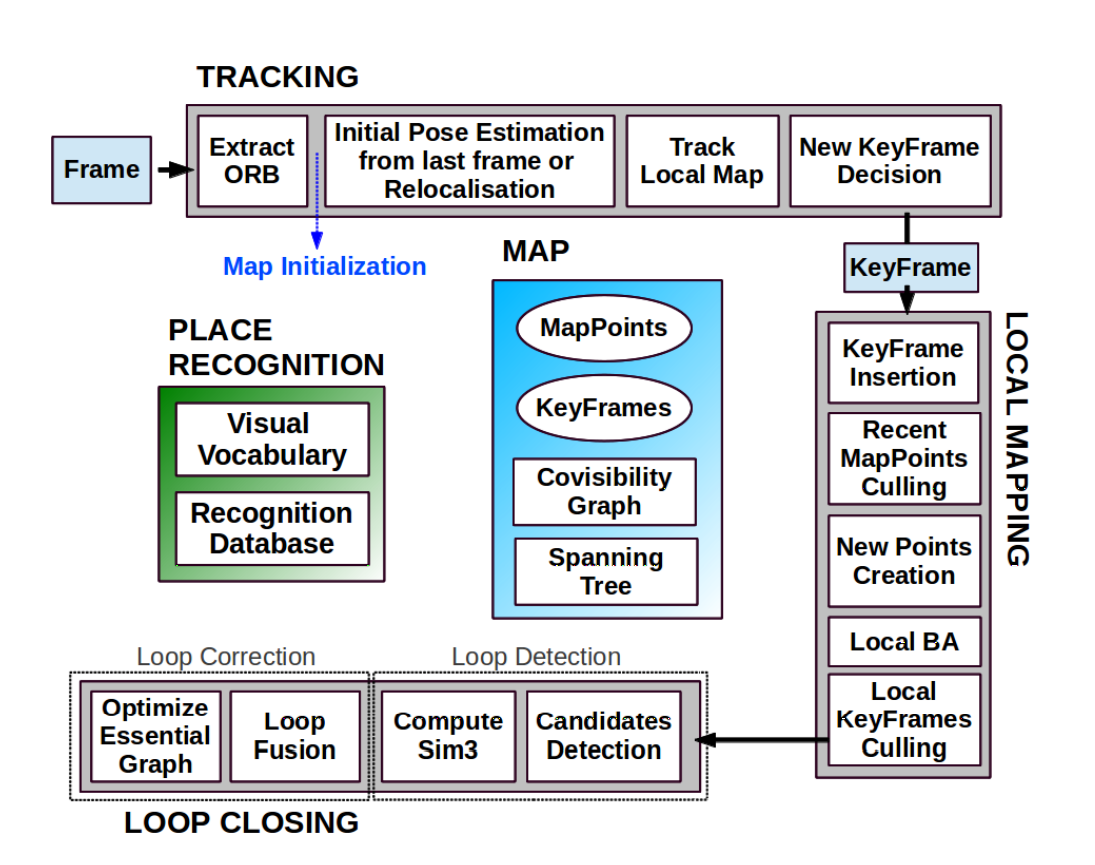
\includegraphics[scale=0.6]{orb.png}
	\caption{ORB-SLAM System Übersicht: Tracking, Mapping und Loop Closing. Bildquelle \cite{orbslam_og}.}
\end{figure} 

ORB-SLAM arbeitet mit verschiedenen Threads, um das Tracking, Mapping und Loop Closing parallel auszuführen. 

Der \textbf{Tracking} Thread ist für die Lokalisierung der Kamera zuständig und entscheidet auch, welche Keyframes ausgewählt werden. Keyframes sind die Menge der Frames, die für die Erstellung der Map verwendet werden. Dabei wird mit einem \glqq Survival of the Fittest\grqq{} Ansatz gearbeitet, der die nützlichsten Keyframes findet. Die initiale Positionsschätzung wird durch das Feature Matching zwischen ausgewähltem und vorherigem Keyframe erreicht. Danach wird die aktuelle Position mithilfe eines Bewegungsmodells optimiert, um die korrespondierenden Map Points aus dem Keyframe vorherzusagen und die 3D-Rekonstruktion zu optimieren. Wenn das Tracking eines vorherigen Frames verloren geht, wird ein globaler Lokalisierungsalgorithmus verwendet, um ein neues Keyframe zu finden, das dann wieder mit dem aktuellen Frame verglichen werden kann. Ein erfolgreicher Tracking Schritt resultiert in dem Finden einer Kamerapose und einem initialen Set an Features, aus denen dann eine lokale Karte berechnet werden kann. 

Die \textbf{Map} wird aus den ermittelten Keyframes und den darin enthaltenen Map Points im zweiten Thread erstellt. Wenn ein Keyframe erfasst wird, wird es in einem Graphen abgelegt, der dieses als Node und die gemeinsam beobachteten Map Points in den verschiedenen Keyframes als Verbindungen zwischen den Nodes modelliert. Die Gewichtung der Kanten ist die Anzahl der Map Points, die auf beiden Frames observiert wurden. Um ein unbeschränktes Wachstum des Graphen zu vermeiden, werden Keyframes aussortiert, die im Vergleich zu anderen zu ähnlich sind. Map Points werden ebenfalls aussortiert, wenn sie von zu wenigen Keyframes gleichzeitig erfasst werden. Auf diese Weise können Keyframes sehr großzügig in den Graphen eingefügt und bei Redundanz wieder entfernt werden.

Das \textbf{Loop Closing} wird vom dritten Thread ausgeführt. Wenn erkannt wird, dass ein bestimmter Ort schon einmal besucht wurde, kann der Drift, der sich beim Durchlaufen der Schleife angesammelt hat, korrigiert werden. Bei ORB-SLAM wird die Schleifenerkennung beim Einfügen jedes Keyframes in den Graphen vorgenommen. Dazu wird die Ähnlichkeit zwischen den Keyframes betrachtet, indem ein Ähnlichkeitswert mithilfe der Anwendung des \glqq Bag-of-Words\grqq{} Modells berechnet wird. Wenn ein Keyframe mehr Ähnlichkeiten mit einem neu eingefügten Keyframe aufweist als seine Nachbarn im Graphen, ist es ein Kandidat für die Schleifenschließung. Wenn drei miteinander verbundene Kandidaten gefunden wurden, gilt der Loop als akzeptiert und die Schleife wird geschlossen. Abschließend wird der Graph aktualisiert (vgl. \cite{orbslam_og} S.6-8, \cite{orb_slam} S.4-5).


\section{Structure from Motion}

Structure from Motion (SfM) ist ein Oberbegriff unter dem verschiedene Verfahren zusammengefasst werden können. Er steht für die gleichzeitige Schätzung der Struktur einer dreidimensionalen Szene und der Bewegung des Sensors in dieser Szene, erstellt aus mehreren überlappenden Bildern einer Szene (siehe Abbildung 4.5). Die Rekonstruktion der 3D-Struktur der Originalobjekte aus diesen 2D-Bildsequenzen wird dann als SfM bezeichnet. 

\begin{figure}[H]
	\centering
	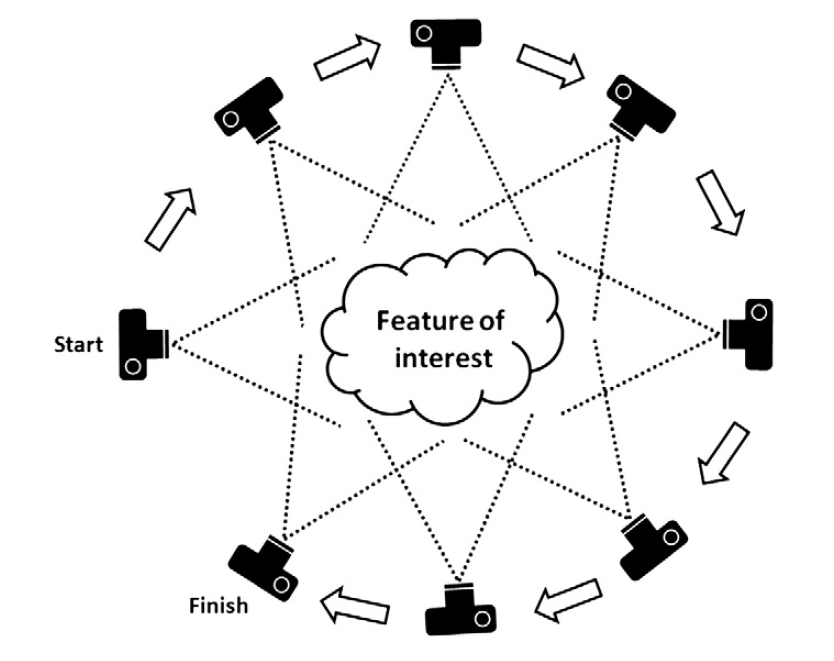
\includegraphics[scale=0.65]{sfm.png}
	\caption{Structure from Motion: Überlappende Fotos zur Rekonstruktion der 3D Szene. Bildquelle \cite{sfm_photo}}
\end{figure}  

Structure from Motion hat in der Computer Vision Community große Beachtung gefunden. Kürzlich vorgestellte Systeme haben erhebliche Fortschritte bei der bildbasierten Modellierung und beim Rendering gemacht. Die meisten Structure from Motion Systeme arbeiten sequentiell, beginnend mit einer kleinen Rekonstruktion aus beispielsweise zwei Bildern und fügen dann schrittweise neue Aufnahmen durch die Pose Estimation der Kamera hinzu. Die Punkte im 3D-Modell werden durch Triangulation oder mit hierarchischen Verfahren eingefügt. \\ Diese SfM Ansätze erfordern je Sequenz die Durchführung des Bündelblockausgleichs, sowie mehrere Iterationen der Ausreißerbeseitigung, um die Ausbreitung von Fehler zu minimieren, während die Rekonstruktion wächst. Für große Datensets ist dies sehr rechenintensiv (vgl. \cite{sfm} S.1).

Structure from Motion ist nicht nur in der Computer Vision vertreten, sondern hat auch in der Photogrammetrie bereits Anwendungsbereiche gefunden. In den letzten Jahrzehnten sind verschiedene Ansätze zur Lösung des SfM Problems entstanden, wie die \glqq Maximum likehood estimation\grqq{}, \glqq Kalman und Extended Kalman Filter\grqq{}, \glqq Particle Filter\grqq{} oder das \glqq Hidden Markov Model\grqq{} (vgl. \cite{efficient_bundle} S.5).

SfM unterscheidet sich von der herkömmlichen Photogrammetrie, indem die Geometrie der Szene, die Kameraposition und die Ausrichtung automatisch ohne die Kenntnis von a priori definierten 3D-Zielen berechnet werden kann (vgl. \cite{sfm_photo} S.301).

\section{Weitere Verfahren - SLAM mit Stereo Kameras}

Visual SLAM kann mit nur einer monokularen Kamera durchgeführt werden. Dies ist die günstigste und kleinste mögliche Sensoranordnung. Das Problem dabei ist jedoch, dass Tiefeninformationenen in solch einem System nicht erfasst werden können. Dadurch sind der Maßstab der erstellten Map, sowie die geschätzte Trajektorie unbekannt. Weiterhin benötigt ein solches System Mehrbildansichten oder Filtertechniken, um die Generierung der initialen Map zu ermöglichen, da diese nicht vom ersten Frame an trianguliert werden kann. Weiterhin ist monokulares SLAM einem Drift ausgesetzt, der regelmäßig korrigiert werden muss. Das Tracking der Umwelt kann auch bei reiner Rotation des Geräts, ohne eine Positionsänderung zu vollziehen, bei der Erkundung versagen. Durch den Einsatz von Stereo- oder RGB-D-Kameras können diese Probleme gelöst werden, was eine zuverlässigere Lösung für das SLAM Problem darstellt (vgl. \cite{orbslam2} S.1).

\subsection{Stereo SLAM}

Die meisten modernen Stereo SLAM Systeme sind Keyframe basiert und führen die Optimierung in einem lokalen Bereich mithilfe des Bündelblockausgleichs durch, um Stabilität zu erreichen. Dabei werden die Tiefeninformationen aus den Differenzen der Bilder, der typischerweise nebeneinander liegenden Kameras, berechnet. \\ Beispiele für Stereo SLAM sind etwa \glqq Conditionally Independet Divide and Conquer EKF-SLAM\grqq{} (Paz et al. 2008), \glqq RSLAM\grqq{} (Mei et al. 2011), \glqq Stereo parallel tracking and mapping (S-PTAM)\grqq{} (Pire et al. 2015) oder \glqq Large-scale direct SLAM (LSD-SLAM)\grqq{} (Engel et al. 2015) (vgl. \cite{orbslam2} S.2).

\subsection{RGB-D SLAM}

Durch die Entwicklung von RGB-D Kameras, die neben den Farbinformationen noch einen extra Kanal für die Tiefeninformationen des Bildes bereitstellen, haben sich verschiedenste SLAM Ansätze entwickelt. Dies hat sich jedoch erst nach dem Aufkommen von RGB-D Kamerasystemen ergeben. Die ersten Ansätze von RGB-D SLAM basierten auf der Entwicklung der Kinect von Microsoft. Das System heißt KinectFusion und wurde von Newcombe et al. (2011) eingeführt. Bei diesem Verfahren wurden alle Tiefeninformationen zu einem volumetrisch dichten Modell verschmolzen, mit dem dann die Kameraposition mittels ICP (Iterative Closest Point) verfolgt wird. Dieses System war aufgrund seiner volumetrischen Repräsentation auf kleine Arbeitsbereiche beschränkt, was auch durch das Fehlen von Loop Closing bedingt wurde. Weitere Beispiele für RGB-D SLAM Verfahren sind etwa \glqq Kintinous\grqq{} (Whelan et al. 2015), das Open Source RGB-D SLAM (Endres et al. 2014), \glqq DVO-SLAM\grqq{} (Kerl et al. 2013) oder \glqq ElasticFusion\grqq{} (Whelan et al. 2016) (vgl. \cite{orbslam2} S.2-3).

\subsection{ORB-SLAM2}

ORB-SLAM2 ist die Erweiterung von ORB-SLAM für Stereo oder RGB-D Kameras und verarbeitet die merkmalsbasierten Eingaben in einem Extraktionsschritt vor, um Merkmale an bestimmten Keypoints zu finden (siehe Abbildung 4.6. (b)). Die Eingabebilder werden nach der Vorverarbeitung verworfen und alle Operationen des Systems basieren nur noch auf den extrahierten Features, sodass das System unabhängig von Stereo oder RGB-D Sensor arbeitet. ORB-SLAM2 kann aber genauso monokularen Input verarbeiten. Anders als die in Kapitel 4.7.2. genannten Methoden arbeitet ORB-SLAM2 mit dem Bündelblockausgleich und baut eine globale Rekonstruktion auf. Das Ziel ist es, eine stabile, schnelle Methode zu liefern, die auf den meisten Standard CPUs arbeiten kann und die statt einer detailreichen, dichten Rekonstruktion eher auf eine langfristige und konsistente Lokalisierung abzielt (vgl. \cite{orbslam2} S.2-3).

\begin{figure}[H]
	\centering
	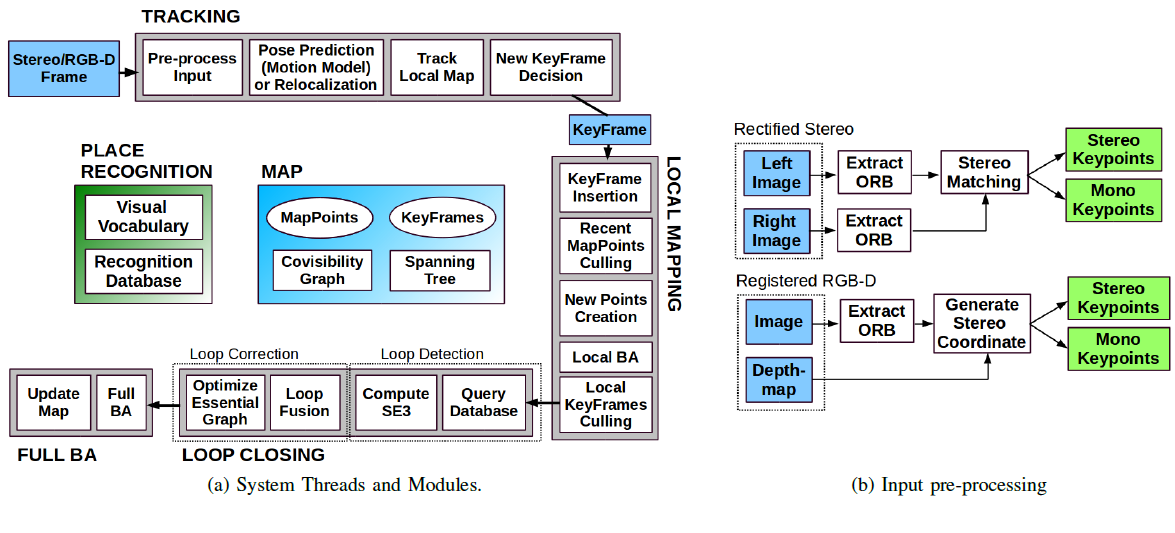
\includegraphics[scale=0.56]{orbslam2.png}
	\caption{(a) Gesamtaufbau der drei Verarbeitungsthreads in ORB-SLAM2 (b) Vorverarbeitung des Stereo oder RGB-D Kamerabildes. Bildquelle \cite{orbslam2}}
\end{figure}  




















